\section{Mixed Max Cut}

\textbf{Definition}: Ein Schnitt in $G=(V,E)$ ist eine Kantenmenge $C\subseteq E$, die von einer Knotenmenge $A\subseteq V$ folgendermaßen induziert wird:
$$C=\{uv\in E\mid |A\cap\{u,v\}|=1\}$$
$C$ enthält also genau die Kanten, die genau einen Endpunkt in $A$ haben.\\

\begin{center}
	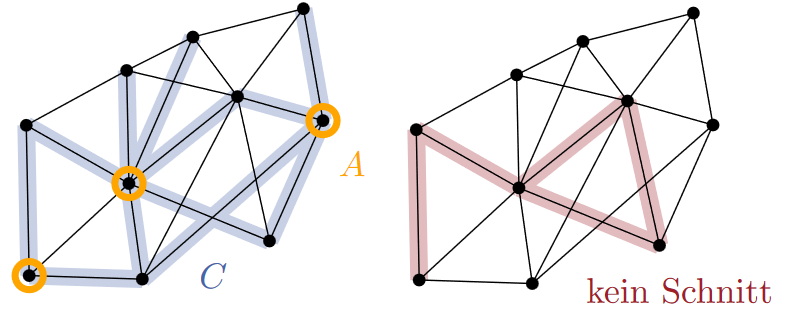
\includegraphics[width=0.4\textwidth]{images/cut.png}
\end{center}
\pagebreak

\texttt{MIXED-MAX-CUT}: 
\begin{itemize}
	\item \textbf{Gegeben}: Graph $G=(V,E)$ und Gewichtsfunktion $w\colon E\rightarrow\R$
	\item \textbf{Gesucht}: Schnitt $C\subseteq E$ mit $w(C)=\sum\limits_{e\in C} w(e)$ maximal und $C\neq\emptyset$
\end{itemize}
\bigskip
\textbf{Satz}: \texttt{MIXED-MAX-CUT} ist auf planaren Graphen polynomiell lösbar.

\textit{Beweis}: Gegeben einen Graphen $G_0=(V, E_0)$ und $w\colon E_0\rightarrow\R$.
\begin{enumerate}
	\item Trianguliere $G_0$ zu $G=(V,E)$ und setze $w(e)=0$ für jede Kante $e\in E\setminus E_0$
	\begin{center}
		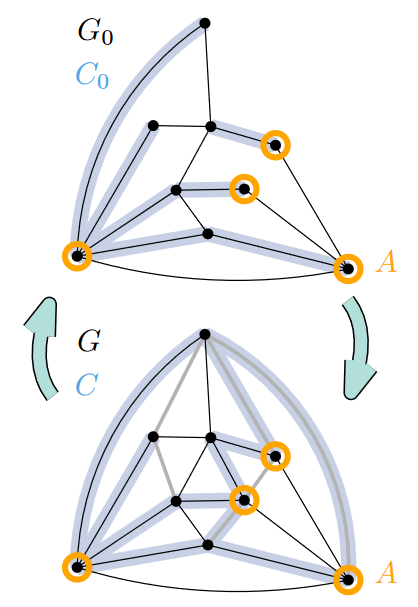
\includegraphics[width=0.19\textwidth]{images/mmc-1.png}
	\end{center}
	\textbf{Beobachtung}: Für Schnitt $C$ in $G$ und $C_0=C\cap E_0$ in $G_0$ sind äquivalent:
	\begin{itemize}
		\item $A\subseteq V$ induziert $C_0\subseteq E_0$ in $G_0$
		\item $A\subseteq V$ induziert $C\subseteq E$ in $G$
	\end{itemize}
	Außerdem gilt $w(C_0)=w(C)$, also reicht es im Folgenden den triangulierten Graphen anzuschauen. 
	
	\textbf{Achtung}: $C_0=\emptyset$ könnte gelten! Das wird später behoben.
	
	\item Betrachte Dualgraph $G^*=(F,E^*)$ von $G=(V,E)$.
	\begin{itemize}
		\item Setze $w(e^*)=w(e)$ für alle $e\in E$
		\item $G^*$ ist 3-regulär, d.h. jeder Knoten hat Grad 3
		\item Für jede Kantenmenge $C^*\subseteq E^*$ hat jeder Dualknoten 0, 1, 2 oder 3 inzidente Kanten in $C^*$
	\end{itemize}
	\begin{center}
		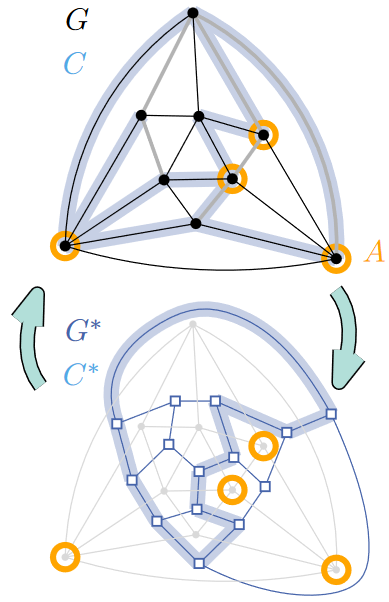
\includegraphics[width=0.18\textwidth]{images/mmc-2.png}
	\end{center}
	
	\textbf{Definition}: Kantenmenge $X\subseteq E^*$ heißt \textbf{gerade}, wenn jeder Knoten zu gerade vielen Kanten in $X$ inzident ist.
	
	\textbf{Lemma}: Sei $G = (V , E)$ trianguliert, $G^*$ zu $G$ dual. Dann gilt:
	$$C\subseteq E \text{ ist Schnitt} \iff C^*\subseteq E^* \text{ ist eine gerade Kantenmenge}$$
	Außerdem ist $w(C)=w(C^*)$.
		
	\textit{Beweis}: 
	\begin{itemize}
		\item \enquote{$\Rightarrow$}: Sei $C\subseteq E$ Schnitt in $G$ induziert von $A\subseteq V$. Sei $f\in V(G^*)$ und $e_1^*,e_2^*,e_3^*$ seine drei inzidenten Kanten. Betrachte das zu $f$ zugehöriges Dreieck $v_1,v_2,v_3$ in $G$.
		\begin{center}
			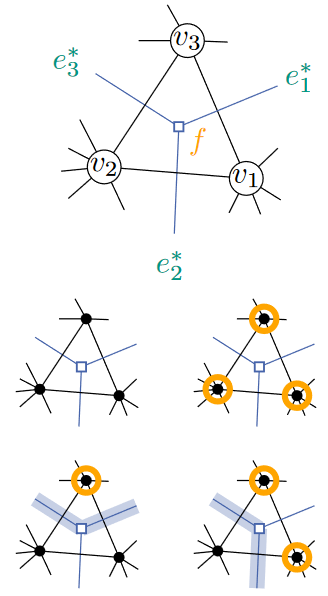
\includegraphics[width=0.2\textwidth]{images/mmc-3.png}
		\end{center}
		\begin{itemize}
			\item Ist $|A\cap \{v_1,v_2,v_3\}|=0,3$, dann $|C^*\cap\{e_1^*,e_2^*,e_3^*\}|=0$
			\item Ist $|A\cap \{v_1,v_2,v_3\}|=1,2$, dann $|C^*\cap\{e_1^*,e_2^*,e_3^*\}|=2$
		\end{itemize}
		
		Also ist $C^*$ gerade.
		
		\item \enquote{$\Leftarrow$}: Sei $C^*\subseteq E^*$ eine gerade Kantenmenge in $G^*$. Dann hat jeder Dualknoten 0 oder 2 inzidente Kanten in $C^*$, also ist $C^*$ eine disjunkte Vereinigung von Kreisen und isolierten Punkten $C_1,\ldots,C_k$. Sei nun 
		$$A=\{v\in V\mid v \text{ ist im Inneren von ungerade vielen Kreisen}\}$$
		Dann gilt:
		$$
		\begin{aligned}
			& e\in E \text{ ist in } C \\
			\Leftrightarrow\; & e^*\in C^*\\
			\Leftrightarrow\; & e^*\in C_i \text{ für ein } i\in\{1,\ldots,k\}\\
			\Leftrightarrow\; & \text{Endpunkte von } e \text{ liegen auf verschiedenen Seiten von } C_i\\
			\Leftrightarrow\; & \text{Genau einer der Endpunkte von } e \text{ ist in } A
 		\end{aligned}
		$$
		Also ist $C$ ein Schnitt und wird von $A$ induziert.
	\end{itemize}
	\begin{center}
		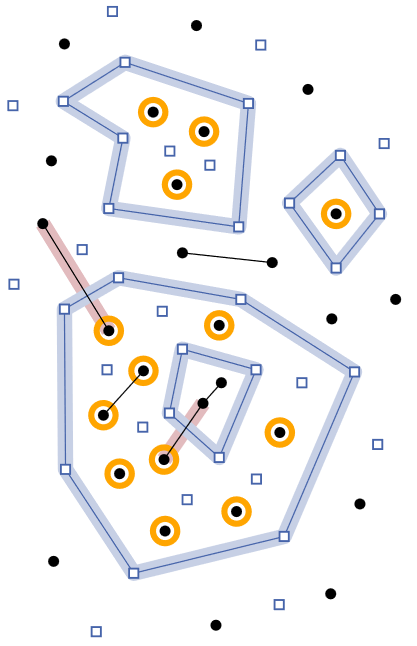
\includegraphics[width=0.2\textwidth]{images/mmc-4.png}
	\end{center}

	Wir suchen jetzt also eine gewichtsmaximale gerade Kantenmenge $C^*$ in $G^*$. Das heißt, jeder Knoten hat Grad 0 oder 2 in $C^*$.
	
	\item Modifiziere $G^*=(F,E^*)$ zu $G'=(V',E')$ wie folgt:
	\begin{center}
		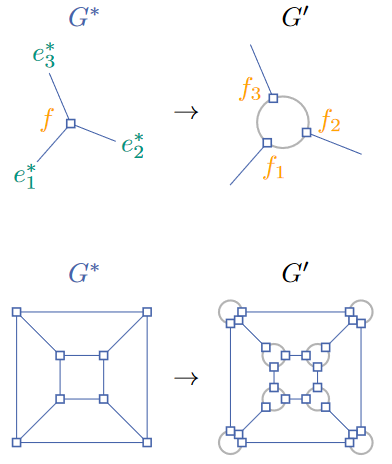
\includegraphics[width=0.3\textwidth]{images/mmc-5.png}
	\end{center}
	Ursprüngliche Kanten behalten ihr Gewicht und neue Kanten erhalten Gewicht 0. $G'$ ist wieder planar und 3-regulär.\\
	
	\textbf{Definition}: Sei $k\in\N$ eine Zahl. Eine Kantenmenge $X\subseteq E$ heißt \textbf{$\mathbf{k}$-Faktor}, wenn jeder Knoten zu genau $k$ Kanten in $X$ inzident ist.
	\begin{itemize}
		\item 1-Faktoren heißen auch \textbf{perfekte Matchings}
	\end{itemize}

	\textbf{Lemma}: 
	\begin{itemize}
		\item Für jede gerade Menge $C^*\subseteq E^*$ existiert ein 2-Faktor $C'\subseteq E'$ mit $C'\cap E^*=C^*$
		\item Für jeden 2-Faktor $C'\subseteq E'$ ist $C^*=C'\cap E^*$ eine gerade Menge
		\item Es gilt $w(C')=w(C^*)$
	\end{itemize}
	\pagebreak
	
	\textit{Beweis}: 
	\begin{center}
		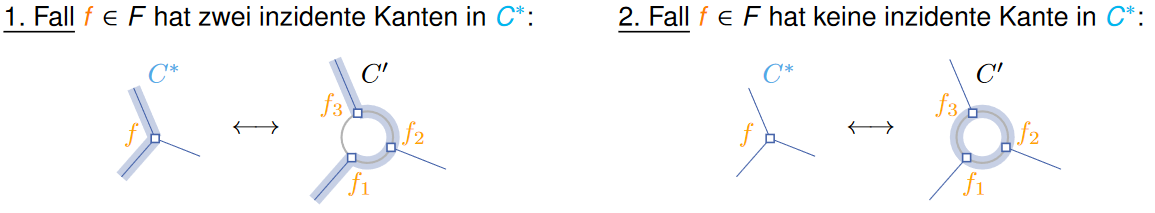
\includegraphics[width=0.8\textwidth]{images/mmc-6.png}
	\end{center}

	Wir suchen jetzt also einen gewichtsmaximalen 2-Faktor $C'$ in $G'$.
	
	\item Betrachte 1-Faktoren (perfekte Matchings) statt 2-Faktoren.
	\begin{itemize}
		\item Da $G'$ 3-regulär ist, ist das Komplement eines 2-Faktors $C'$ in $G'$ ein perfektes Matching $M$. $$M=E'-C'$$
		\item 2-Faktor $C'$ ist gewichtsmaximal genau dann, wenn das komplementäre perfekte Matching $M$ gewichtsminimal ist
		$$w(M)=w(E)-w(C')$$
	\end{itemize}
	\begin{center}
		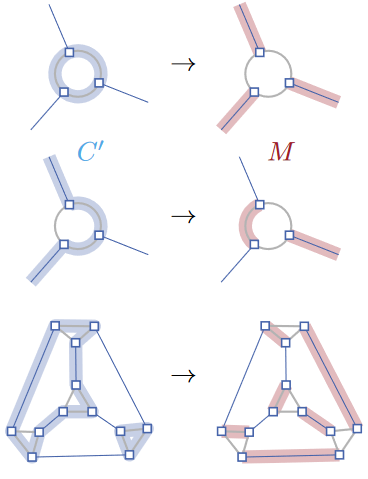
\includegraphics[width=0.2\textwidth]{images/mmc-7.png}
	\end{center}
\end{enumerate}
Damit haben wir einen Algorithmus angegeben, der das Problem löst. Im Folgenden betrachten wir die Laufzeit.\\

\textbf{Satz}: In planaren Graphen können gewichtsminimale perfekte Matchings in $\mathcal{O}(n^\frac{3}{2}\log n)$ berechnet werden.

\textit{Beweis}: Reduziere auf gewichtsmaximales Matching.
\begin{itemize}
	\item $w'(e)\coloneqq -w(e)$, d.h. maximal bezüglich $w'$ $\iff$ minimal bezüglich $w$
	\item $w''(e)\coloneqq W+w'(e)$ für großes $W>|V|\cdot\max\limits_{e\in E'} (|w'(e)|)$, also hat max. Matching bzgl. $w''$ die größtmögliche Anzahl Kanten. Damit sind gewichtsmaximale Matchings bzgl. $w''$ perfekt.
	\item Max. Matchings bzgl. $w''$ entsprechen also genau den min. perfekten Matchings bezüglich $w$.
	\item Da \texttt{MAX MATCHING} in $\mathcal{O}(n^\frac{3}{2}\log n)$ ist, ist der Satz bewiesen.
\end{itemize}
\bigskip
Nun muss nur noch $C_0\neq\emptyset$ sichergestellt werden.
\begin{itemize}
	\item Für eine Kante $e\in E_0$ wollen wir erzwingen, dass $e\in C_0$
	\item Also soll $e^*$ nicht in $M$ sein:
	\begin{itemize}
		\item Unterteile dafür $e^*$ mit Knoten $b$ und setze für die neu entstandenen Kanten $e_1,e_2$ die Gewichte $w(e_1)=w(e^*)$ und $w(e_2)=0$
		\item Füge Kante $e'=bc$ mit neuem Knoten $c$ hinzu und setze $w(e')=0$
		\item Jedes perfekte Matching muss dann $e'$ enthalten
	\end{itemize}
	\begin{center}
		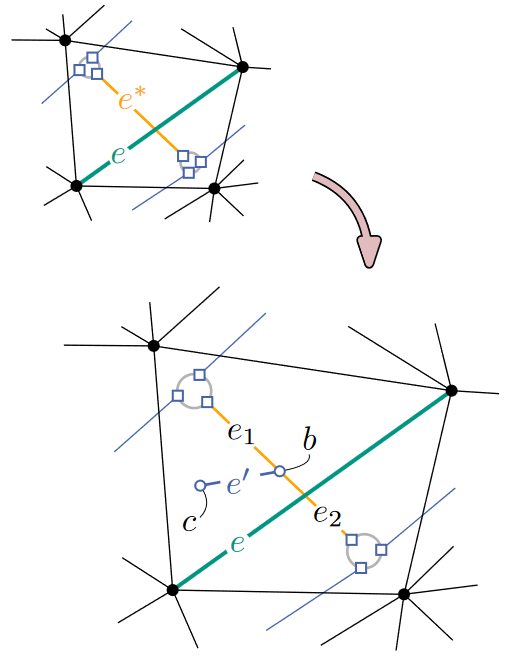
\includegraphics[width=0.3\textwidth]{images/mmc-8.png}
	\end{center}
	\item Um den besten Schnitt zu erhalten, wiederholt man den Vorgang für jede Kante $e\in E_0$
	\item Wir erhalten so die Laufzeit $\mathcal{O}(n^\frac{3}{2}\log n)\cdot\mathcal{O}(n)=\mathcal{O}(n^\frac{5}{2}\log n)$. $\mathcal{O}(n^\frac{3}{2}\log n)$ ist aber möglich!
\end{itemize}

Damit ist der Beweis abgeschlossen. Es folgt eine Übersicht über den Algorithmus.
\begin{center}
	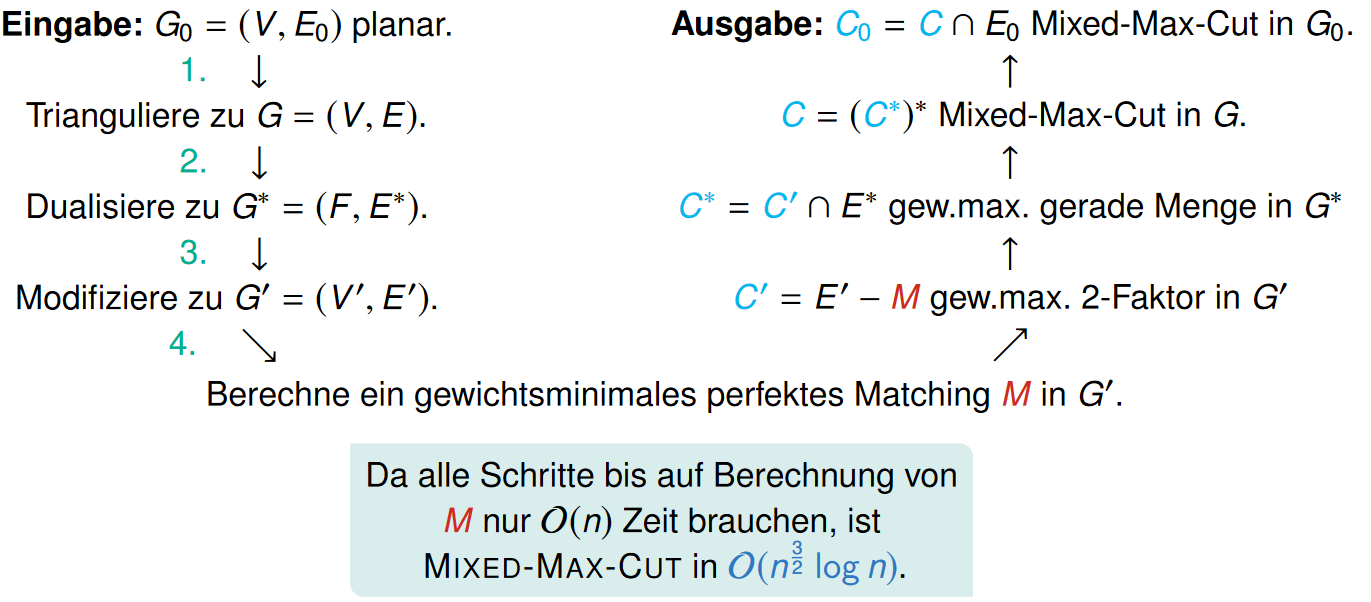
\includegraphics[width=0.8\textwidth]{images/mmc-9.png}
\end{center}
\begin{center}
	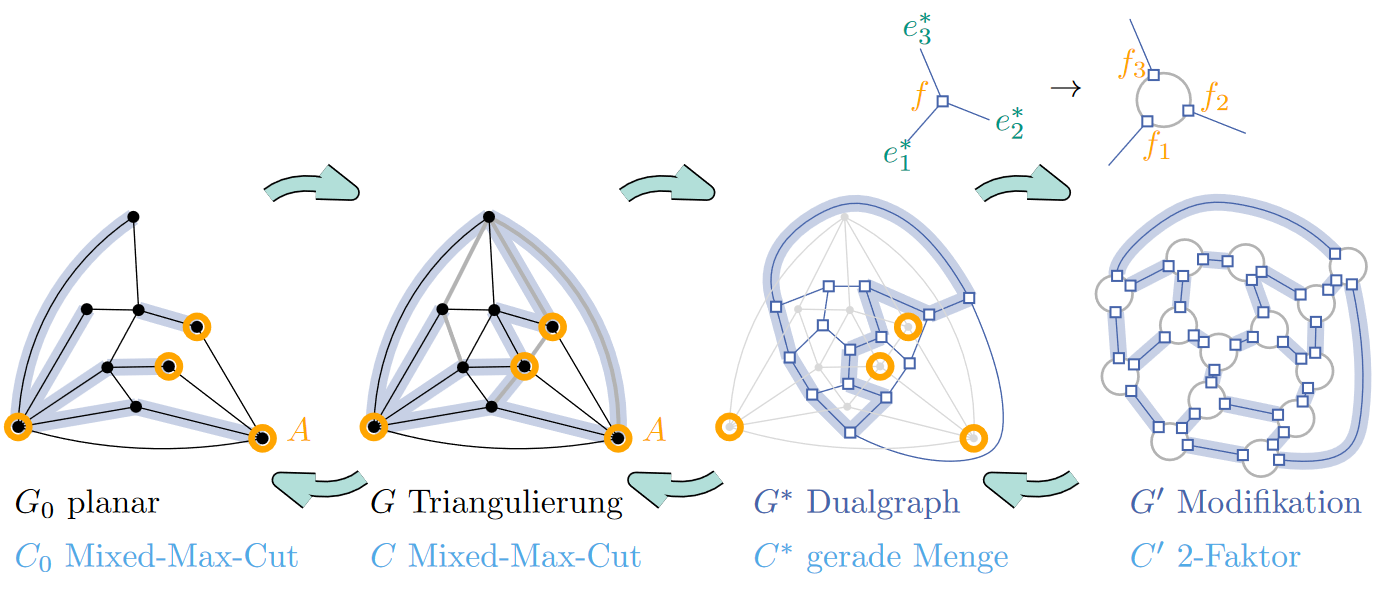
\includegraphics[width=0.8\textwidth]{images/mmc-10.png}
\end{center}